%! Author = wolfram_e_laube
%! Date = 02.04.24

\item [b)]
Plotting the Signals

Figure~\ref{fig:SignalPlot} shows two subplots, one for each frequency. In each subplot, it plots the original signal,
the time-delayed signal (in red dashed lines), and the phase-shifted signal (in green dot-dashed lines,
slightly transparent for better visibility).
The time-delayed and phase-shifted signals are expected to overlap completely,
demonstrating that a time delay is equivalent to a phase shift in the time domain.
\begin{figure}[!ht]
	\centering
	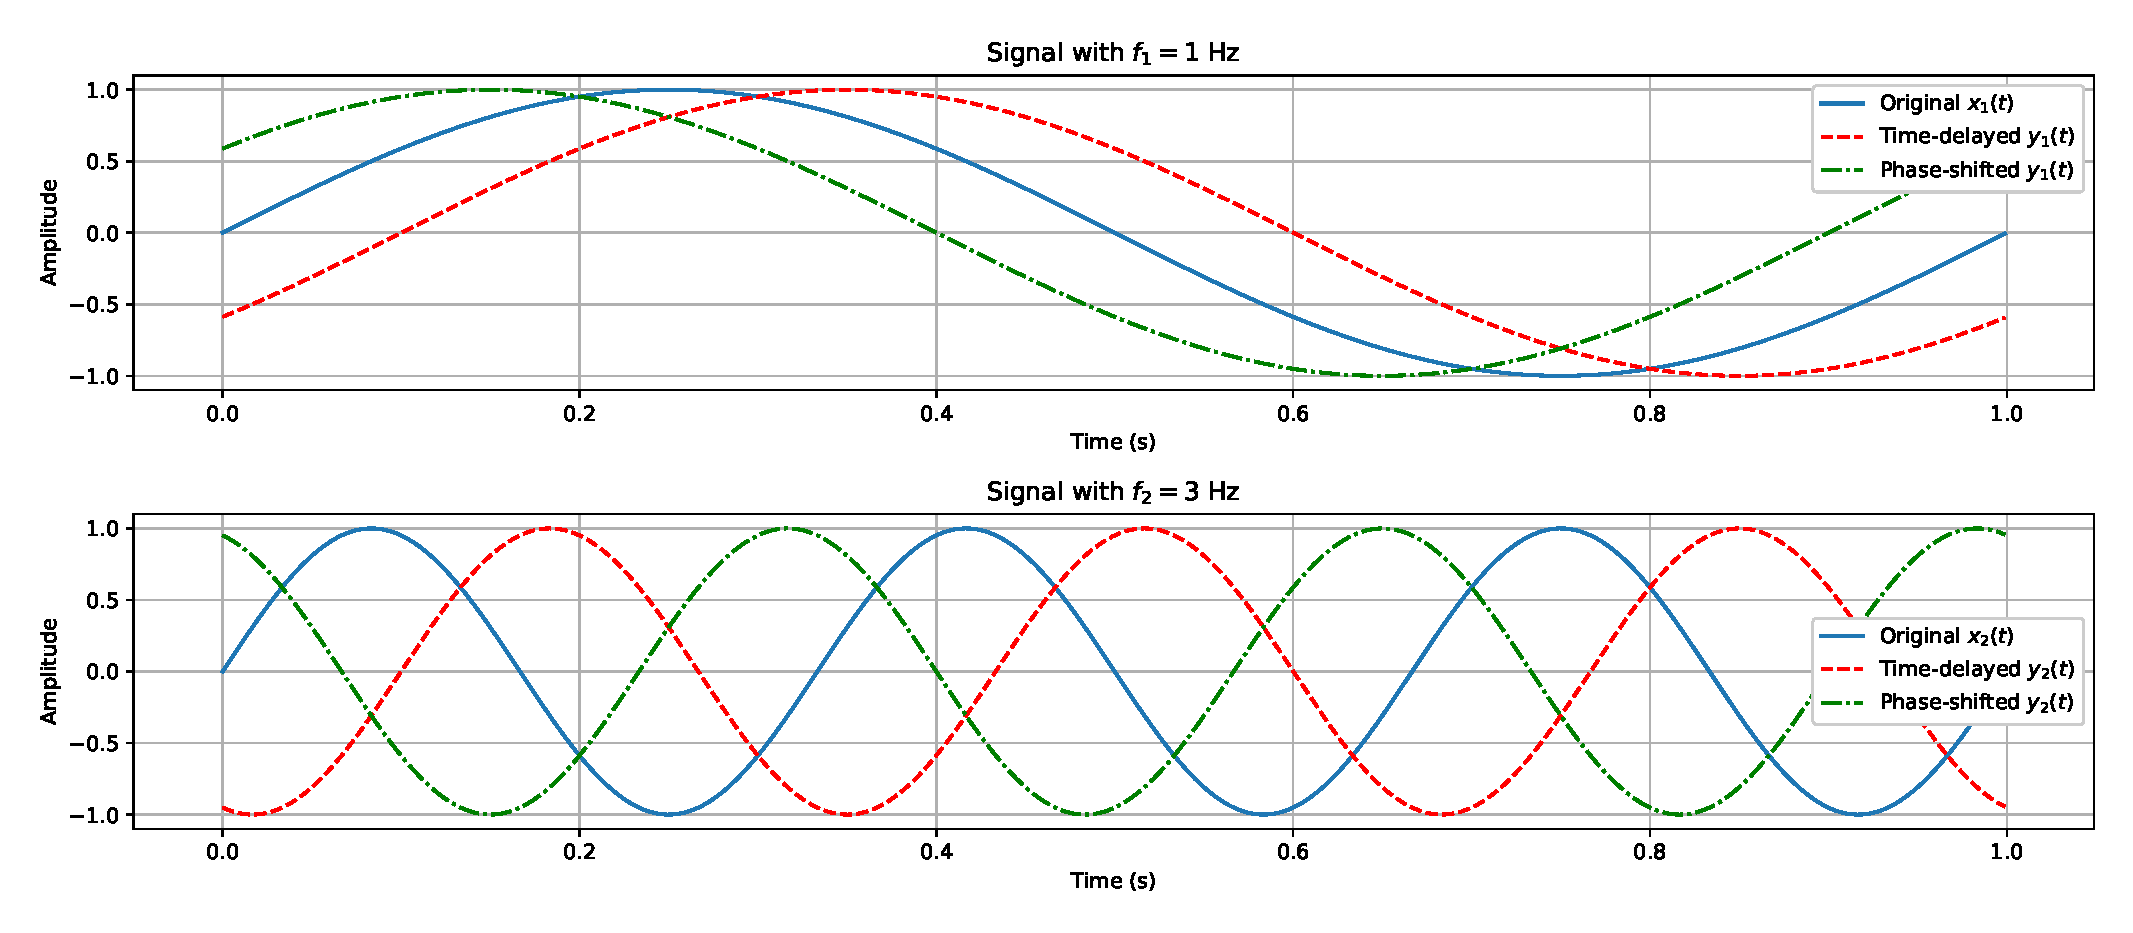
\includegraphics[width=18cm]{ex3_signal_plot.eps}
	\vspace{-0.3cm}
	\caption{Signal Plot.}
	\label{fig:SignalPlot}
	\vspace{-0.1cm}
\end{figure}


